
\chapter{2. Linear PDEs: structured grids}

We start with the Poisson problem because it is the right place to start.  Though it is a cliche in applied mathematics, in solving it we will use key parts of \PETSc.  We will build a structured grid using a \PETSc \pDMDA, assemble a \pMat and some \pVec s in parallel on this grid, and solving in parallel using a \pKSP object.

\section{A Poisson problem on a square}

The \emph{Laplacian} is the most common second-derivative of a function $u(x,y)$ in the plane:
    $$\grad^2 u = \Div(\grad u) = \frac{\partial^2 u}{\partial x^2} + \frac{\partial^2 u}{\partial y^2}.$$

The Laplacian is a linear operator, i.e.~$\grad^2(c_1 u_1 + c_2 u_2) = c_1 \grad^2 u_1 + c_2 \grad^2 u_2$.  When one sees it in a mathematical model, the reason is almost always that there is conservation of some quantity $u$, thus the divergence $\Div$ appears, and that the gradient $\grad u$ is essentially the flux of $u$ \citep{Ockendonetal2003}.  

In the \emph{Poisson equation} the Laplacian of $u$ as a known function.  We will solve not just this one equation, but a \emph{Poisson problem}, on a finite region and including boundary conditions, which determine a unique solution \citep{Evans}.  Let $\mathcal{S}$ be the unit square $[0,1]\times[0,1]$ in the plane.  For this section suppose $f(x,y)$ is continuous.   This is our first Poisson problem:
\begin{marginfigure}
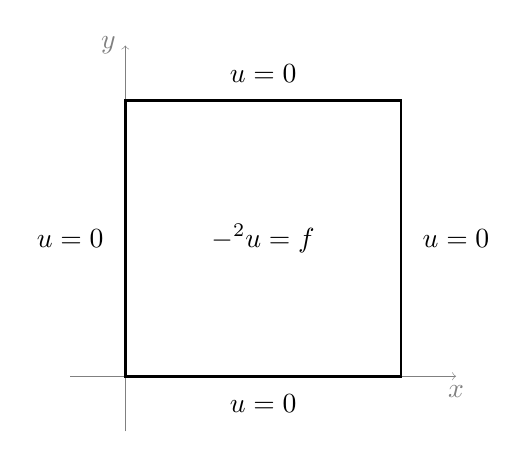
\begin{tikzpicture}[scale=3.5]
  \draw[->,gray,very thin] (-0.2,0.0) -- (1.2,0.0) node[below] {$x$};
  \draw[->,gray,very thin] (0.0,-0.2) -- (0.0,1.2) node[left] {$y$};
  \draw[line width=1.0pt] (0.0,0.0) -- (0.0,1.0) -- (1.0,1.0) -- (1.0,0.0) -- cycle;
  \node at (0.5,0.5) {$- \grad^2 u = f$};
  \node at (0.5,-0.1) {$u = 0$};
  \node at (0.5,1.1) {$u = 0$};
  \node at (-0.2,0.5) {$u = 0$};
  \node at (1.2,0.5) {$u = 0$};
  %\filldraw (0.000000,0.000000) circle (0.500000pt);
\end{tikzpicture}
\caption{Our first, simple goal is to solve the Poisson equation on the unit square $\mathcal{S}$, with homogeneous Dirichlet boundary conditions.}
\label{fig:unitsquare}
\end{marginfigure}
\begin{align}
- \grad^2 u &= f \quad \text{ on } \mathcal{S}, \label{poissonsquare} \\
u &= 0 \quad \text{ on } \partial \mathcal{S}. \notag
\end{align}

Note that the boundary of the unit square, denoted ``$\partial\mathcal{S}$'', is simply union of four (closed) line segments.  The boundary conditions $u=0$ are called ``\emph{homogeneous Dirichlet}.''  Without any boundary conditions, the Poisson equation $-\grad^2 u = f$ alone is not a well-posed problem because if $-\grad^2 u = f$ then also $-\grad^2(u+C)=f$ for any constant $C$; there are many solutions.

This Poisson problem models the distribution of temperature in a conducting object at steady state, the electrostatic potential, the equilibrium distribution from certain random walks, and many other other physical phenomena.  For example, we can illustrate the above comment about the formation of the Laplacian in the context of heat conduction.  In that case the heat flux is $\bq = - \grad u$ (up to a multiplied constant) if $u$ is the temperature, while the steady-state conservation of heat energy balances the divergence of the flux with the heat source $f$, that is $\Div \bq = f$, again up to a multiplied constant.  This is the Poisson equation \eqref{poissonsquare}.  Holding the temperature fixed at zero along the boundary completes the problem.

Problem \eqref{poissonsquare} is also is linear, that is, if $u_1$ and $u_2$ are solutions then affine linear combinations (i.e.~with coefficients that sum to one) are also solutions.  More relevantly to our purposes, \eqref{poissonsquare} is a linear problem in the sense that finite-dimensional approximations of it are simply linear systems.

Such a finite-dimensional approximation comes from applying a \emph{finite difference} method to \eqref{poissonsquare}.  Let

\cinput{structuredlaplacian.c}{Fill matrix entries using \texttt{MatSetValuesStencil}.}{//CREATEMATRIX}{//ENDCREATEMATRIX}{code:structuredlaplacian}

\cinputpart{c2poisson.c}{The right side of equation \eqref{poissongridsystem} comes from differentiating the exact solution, which this method also computes.}{I}{//RHS}{//ENDRHS}{code:ctwopoissonrhs}

\cinputpart{c2poisson.c}{Set up \pDMDA \texttt{da} and \pMat \texttt{A} objects, and assemble the latter by calling \texttt{formlaplacian()}.}{II}{//CREATE}{//ENDCREATE}{code:ctwopoissoncreate}

\cinputpart{c2poisson.c}{Solve using \pKSP, and report on solution.}{III}{//SOLVE}{//ENDSOLVE}{code:ctwopoissonsolve}

\section{Runtime control of linear solver}

FIXME: basic Krylov theory

\section{Time-dependent heat equation}

FIXME: we WON'T do explicit, but it would look like ...

FIXME: use TS for backward-euler
